\section{Macroprudential policy stance}
\subsection{Distance-to-tail approach}
\label{sec:dtt}
The goal of stance assessment is to assist macroprudential policymakers in making informed decisions. The distance-to-tail approach achieves this by quantifying it and disaggregating its sources by the nature.  As was discussed in previous parts, the distance-to-tal metric is simply the difference between the median and tail (5% quantile) of the fitted conditional GDP distribution. \autoref{fig:distance_to_tail_decomposition} depicts Armenia's estimated distance-to-tail over time. An increase of this indicator signals the buildup of vulnerabilities and gives a hint that policy action should supposedly be in tightening direction. What is truly important is the reason behind every move of its metric, as it can be conditioned by factors outside financial system, which, naturally should be out of the focus of macroprudential policy. Put another way, the latter should be concerned by the risks originationand/or amplification within the financial system. That is why, the mechanical rise of this metric is not solely enough for policy action: it should be due to excessive risk accumulation (rise of FCyI) or high stress levels (rise of FCI) in order to be addressed by macroprudential policy. To address this issue, \autoref{fig:distance_to_tail_decomposition}  represents also the decomposition of the distance-to-tail ratio. For the sake of simplicity, some indicators, like capital surplus and liquidity position are not shown.
% Figure 10 misses the description of the yellow line, whether one should look at the right axis or the left one.
\begin{figure*}
    \centering
    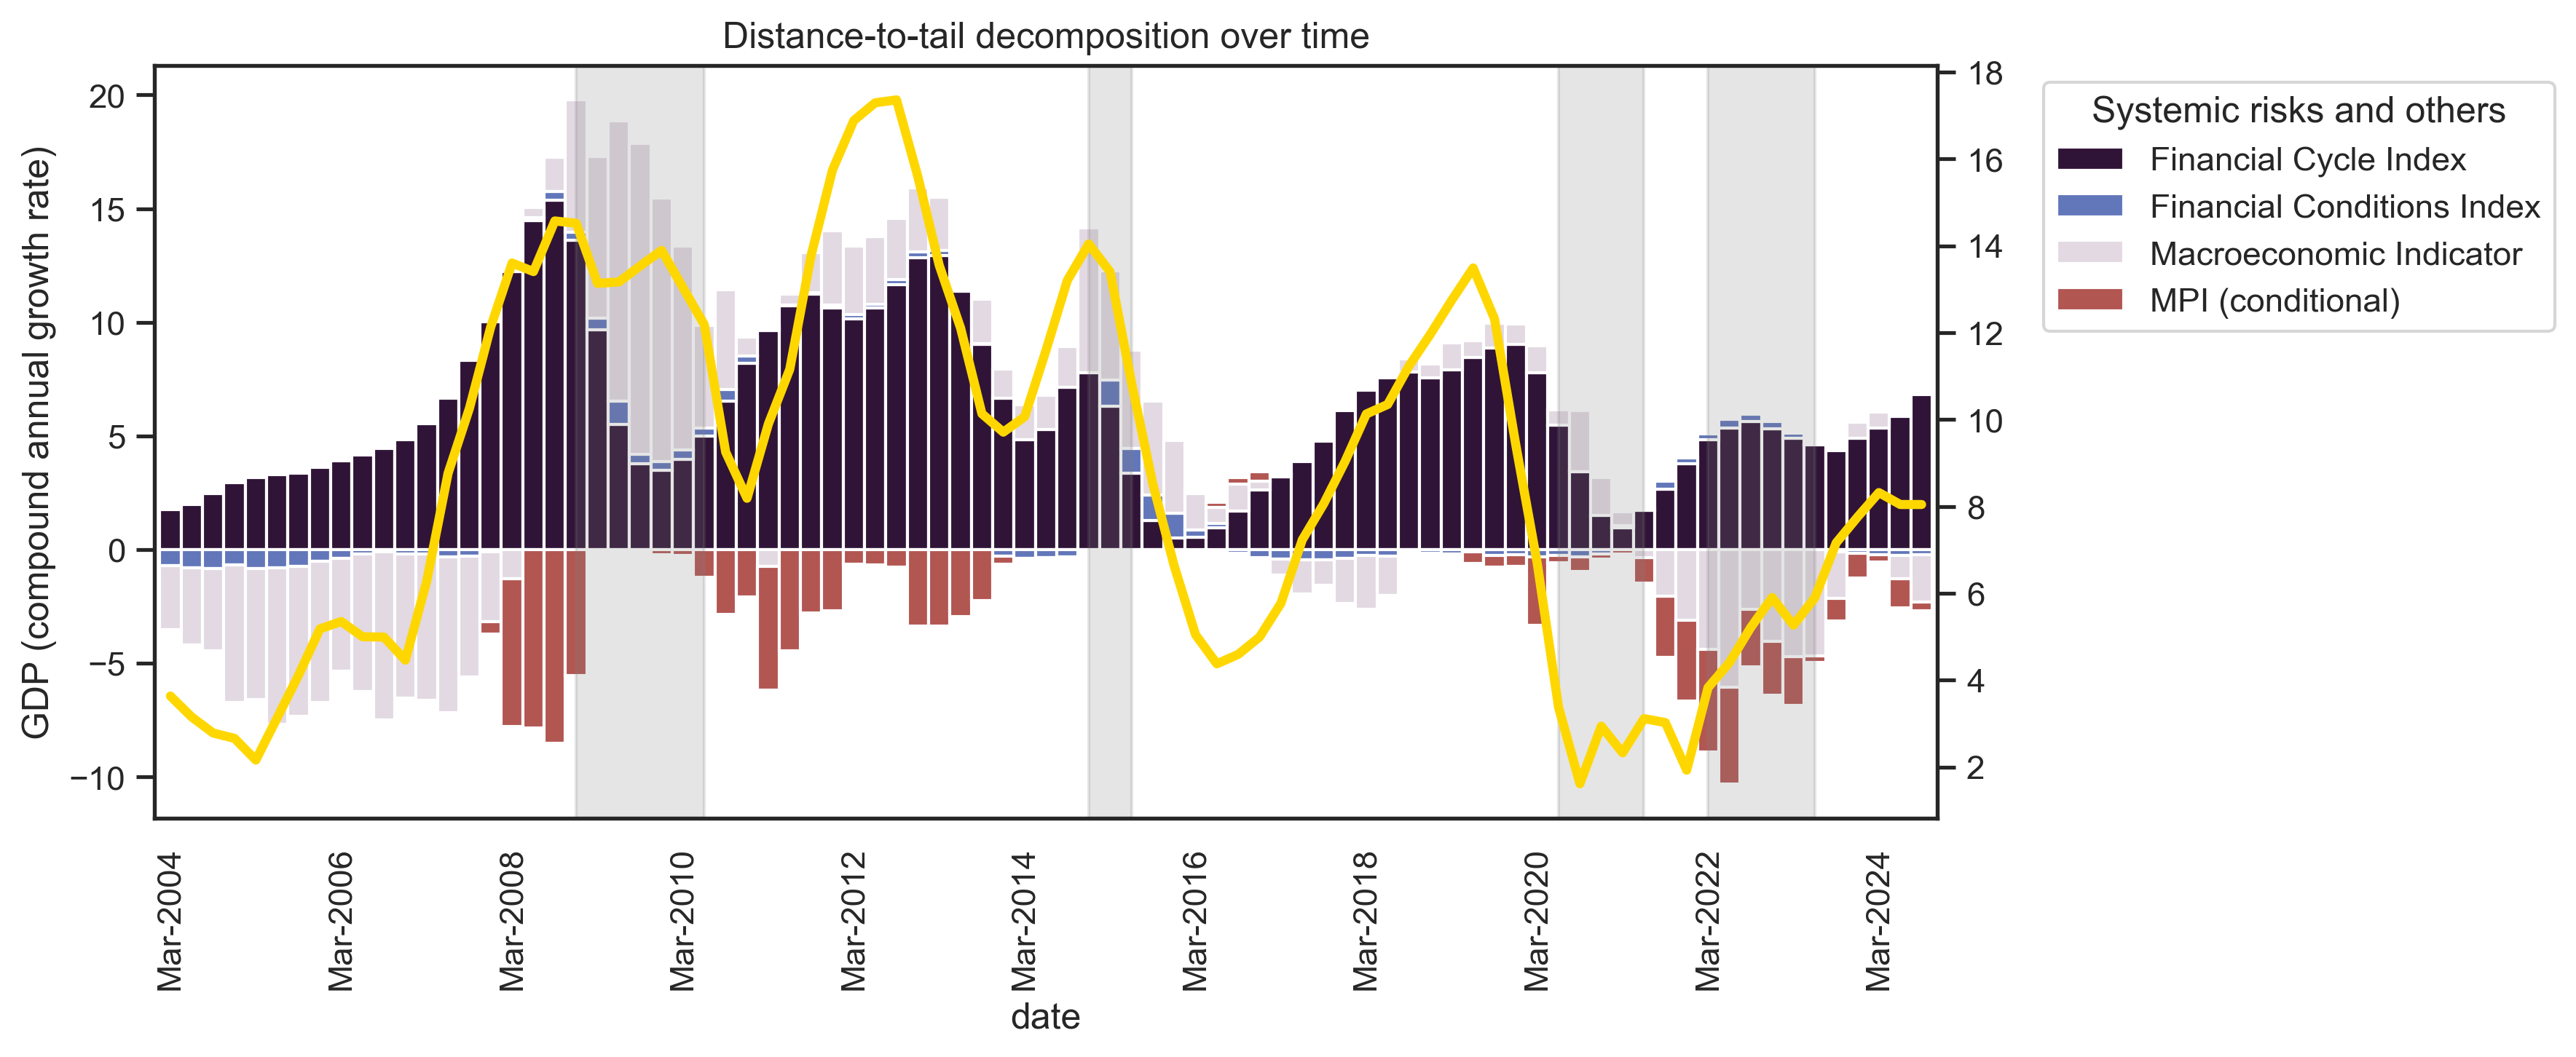
\includegraphics[width=1\textwidth, angle=0]{Figures/distance_to_tail_decomposition.png}    
    \caption{Estimated distance-to-tail over time and decomposition of systemic risks. Vertical areas in grey represent economic disturbances.}
    \label{fig:distance_to_tail_decomposition}%
\end{figure*}
\begin{figure*}
    \centering
    
\includegraphics[width=0.9\textwidth, angle=0]{Figures/distance_to_tail_changes_before_crises.png}  
    \caption{Changes in distance-to-tail and the buildup of systemic risks before major economic disturbances.}
    \label{fig:distance_to_tail_changes_before_crises}%
\end{figure*}
\begin{figure*}
    \centering
    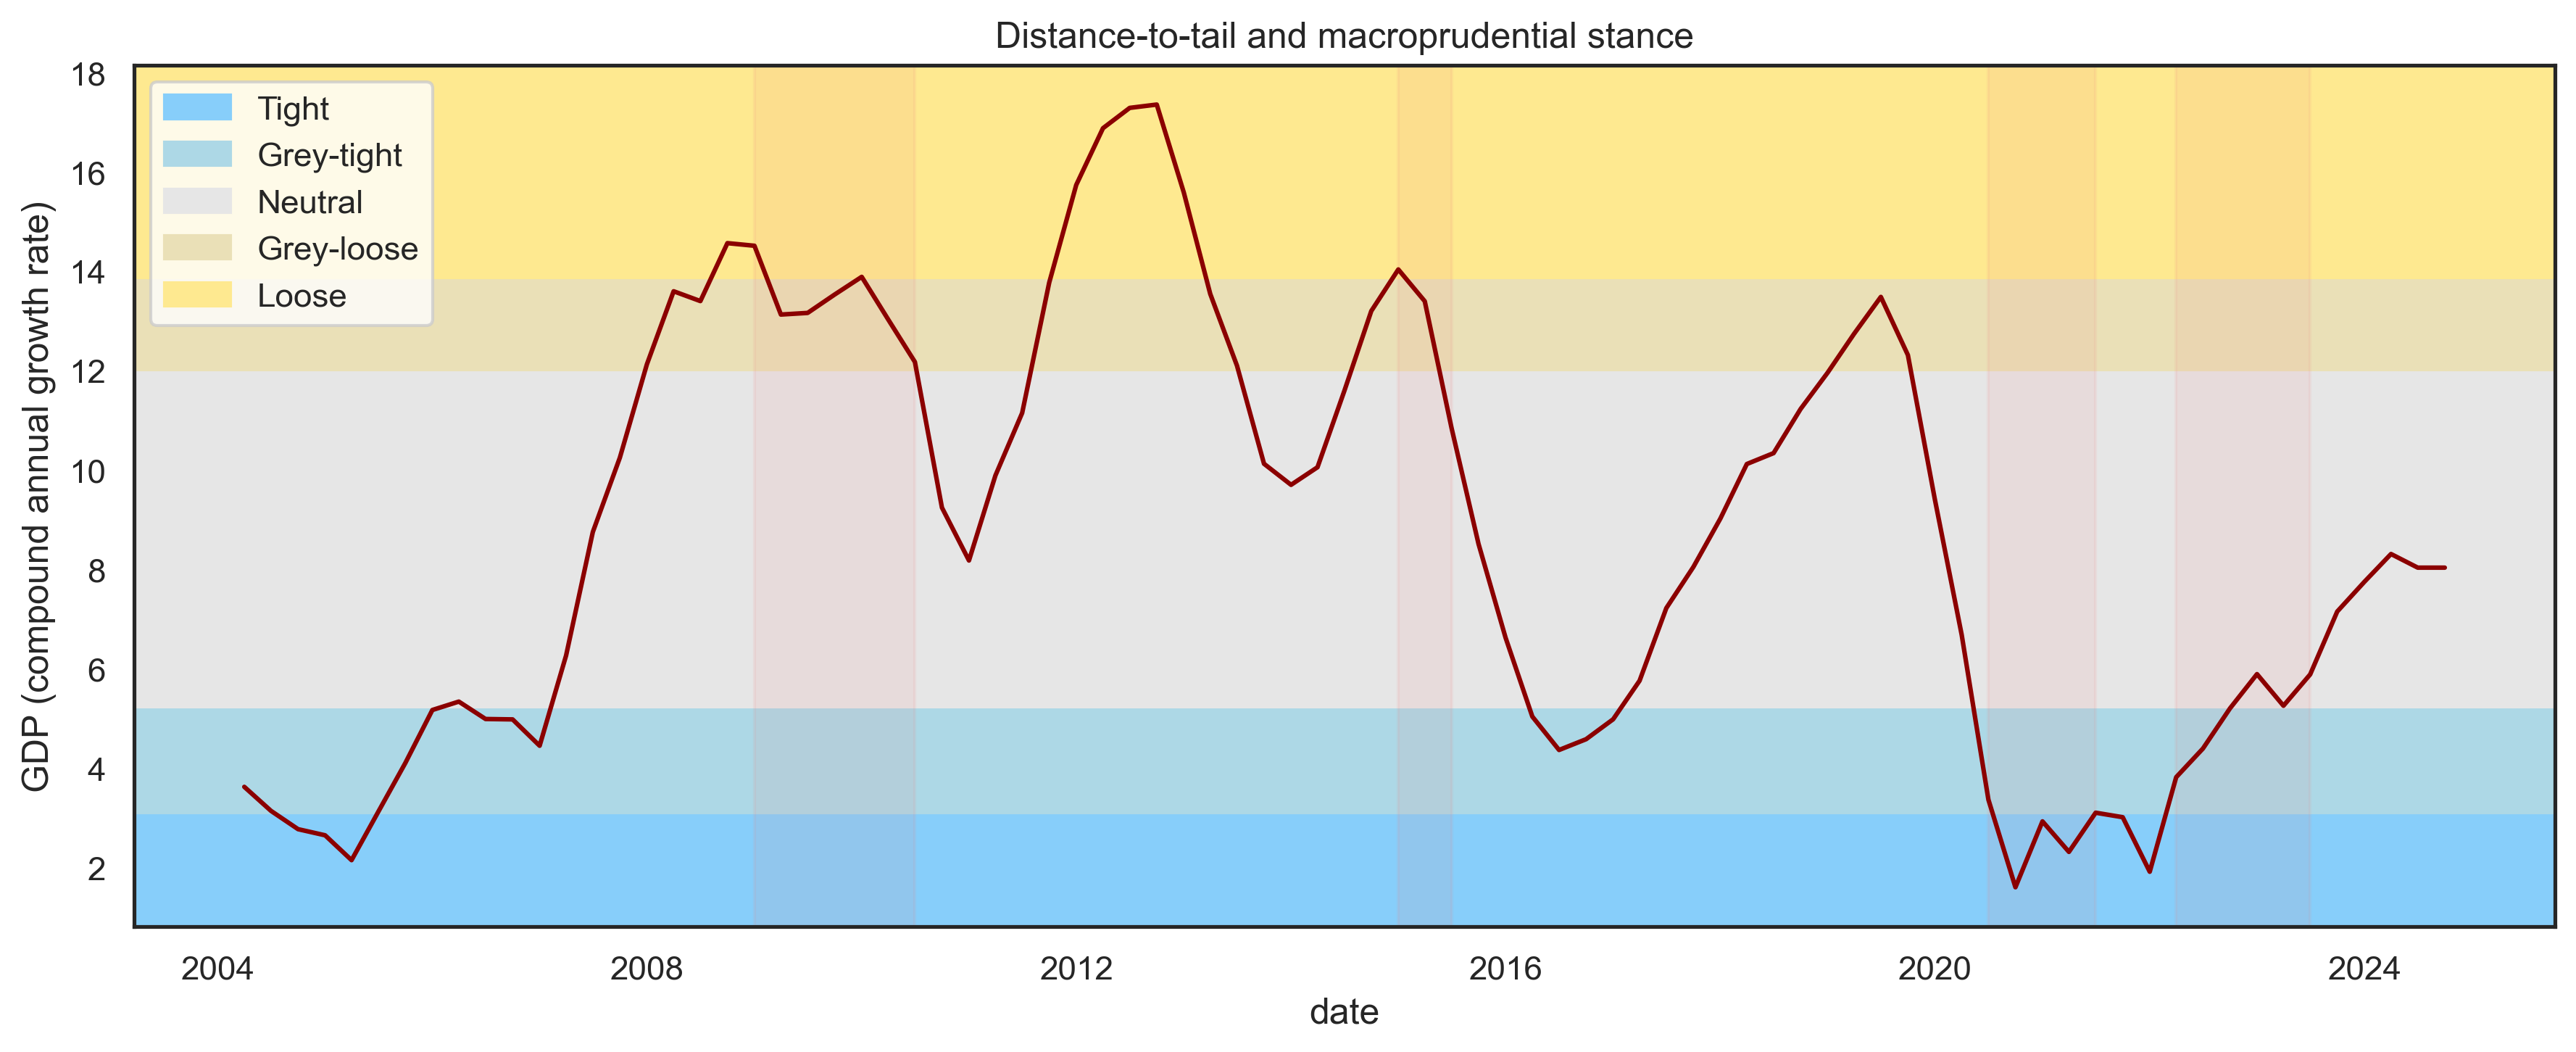
\includegraphics[width=1\textwidth, angle=0]{Figures/distance_to_tail_stance.png}   
    \caption{Estimated distance-to-tail and the macroprudential stance assessment over time. The boundaries describe the 10th, 30th, 70th, and 90th percentiles of the distance-to-tail distribution.}
    \label{fig:distance_to_tail_stance}%
\end{figure*}

The results demonstrate that financial vulnerabilities follow a cyclical pattern, while financial stress tends to have smaller and less persistent impact (it is important to note, that the terms FCyI and FCI also include the interactiuon terms). Macroprudential policy actions mostly contribute to a reduction of risks. Finally, the influence of macroeconomic events on systemic risks is minimal, as they tend to shift the entire GDP growth distribution uniformly, showing little heterogeneity in their effects.

To examine the performance of the distance-to-tail metric for crisis periods we compare systemic risks in Armenia before four major economic disturbances in \autoref{fig:distance_to_tail_changes_before_crises}. Prior to the 2007–2009 financial crisis, there was a significant buildup of financial vulnerabilities, along with the accumulation of other risks that could intensify economic downturns. Indeed, during that period Armenia saw its financial intermediation rising sharply from ~7% in 2005 to 23-24% just before crisis. This rapid growth might have been due to some sort of catch-up process, but also due to rapid risk accumulation, which is correctly pointed by the model result. The decline of this indicator during 2014-2015 Russian oil crisis was conditioned by different set of circumstances, mainly by worsening macroeconomic environment on the one hand, and restrictive macroprudential policy on the other (in the midst of the shock, the CBA sharply raised prvisioning rates of local currency denominated deposits to address local currency devaluation pressures). Before the Covid-19 shock and the Nagorno-Karabakh war, we observe a moderate increase in Financial cycle index, which was abruptly hit by the external shock. Lastly, the period leading up to the Russo-Ukrainian war overlaps with the Nagorno-Karabakh conflict, during which Armenia experienced a downturn in the financial cycle.

The distance-to-tal metric itself does not indicate the threshold where the policymaker should start to act. However, \citep{esrb2021} suggest simple yet effective way to get threshold levels for both directions of the policy, which are based on specific percentiles of its historical series. The stance metric alongside these thresholds is presented in \autoref{fig:distance_to_tail_stance}. When this value exceeds the 12\% distance-to-tail threshold (the 70th percentile), it signals a relatively loose stance, prompting consideration of tightening measures to maintain it at the neutral level. As of 2024Q4, the metric is at the neutral level, suggesting no immediate need for tightening actions. However, the value exhibits an upward trend, indicating growing risks in the system.

A key limitation of the distance-to-tail approach is that the selected threshold is not tied to a measure of the financial system’s resilience, but rather inferred from itself. To test the reliability and robustness of this threshold we use an alternative methodology to derive it, inspired by modern portfolio theory. Using the estimated median and the distance-to-tail (Gap) from the panel quantile regression, we construct an efficient frontier\footnote{For details on the methodology behind the frontier, see \ref{appx:model_results}} across 41 countries, as shown in \autoref{fig:country_cases_that_shape_the_boundary}. 
\begin{figure*}
    \centering
    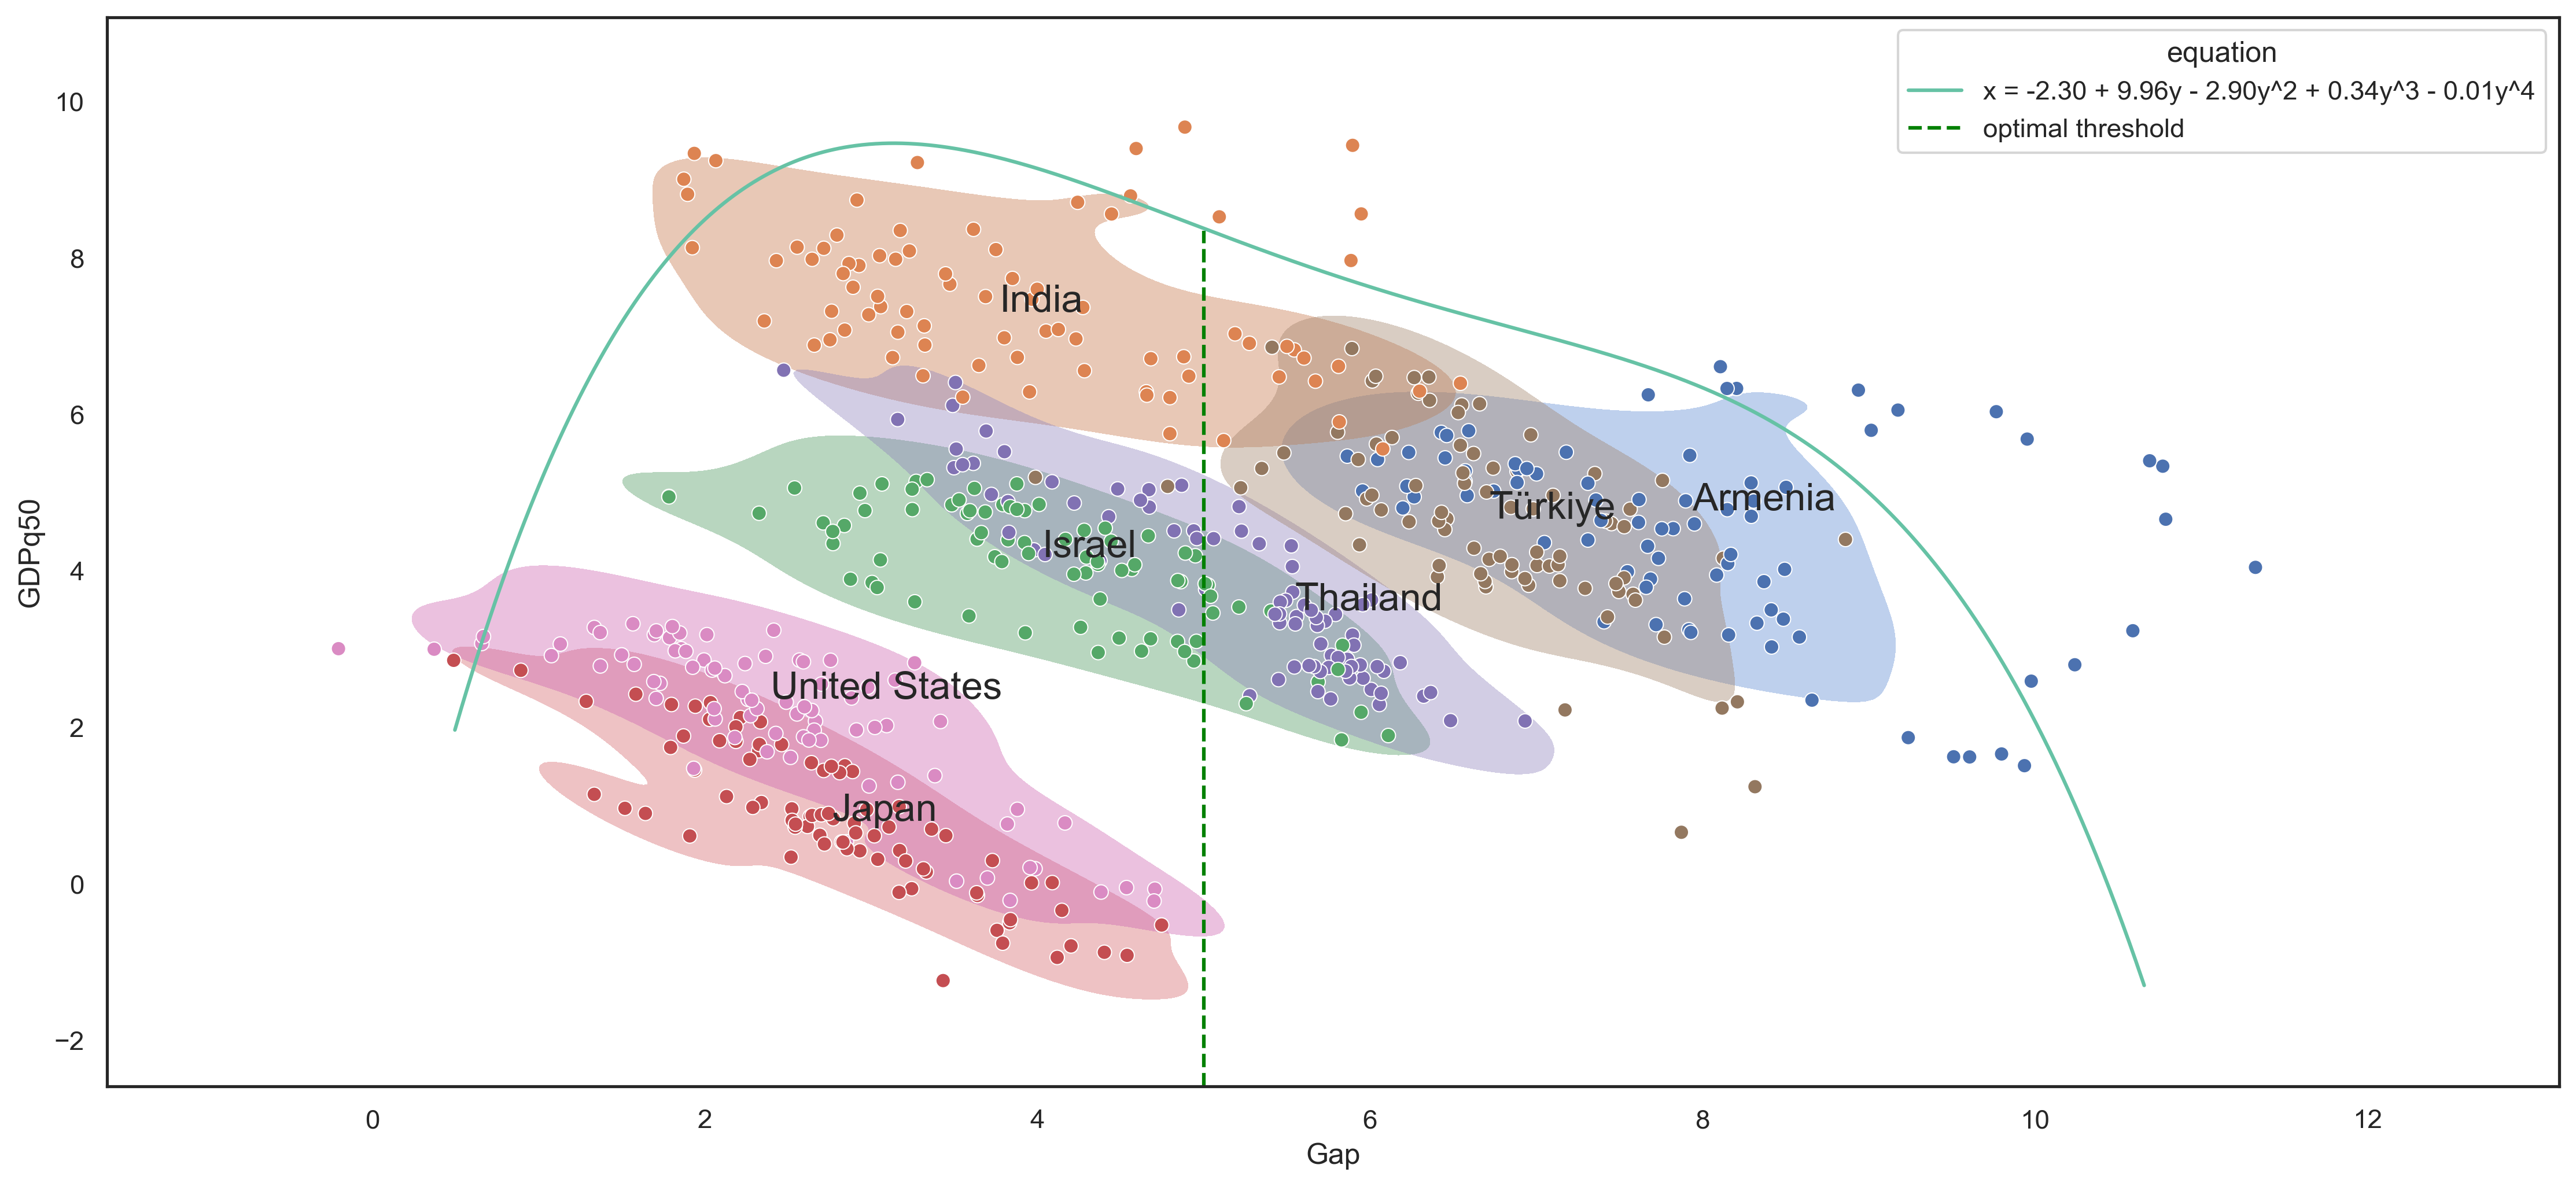
\includegraphics[width=1\textwidth, angle=0]{Figures/country_cases_that_shape_the_boundary.png}   
    \caption{Fitted values for median and the tail from panel estimation and the fitted curve.}
    \label{fig:country_cases_that_shape_the_boundary }%
\end{figure*}

In this context, GDP growth represents each country’s ``portfolio'', with the median as the expected return and the distance-to-tail as the associated risk. The efficient frontier illustrates that beyond a certain threshold, countries that face additional risk do not generate excess returns in proportion to those risks. If we exclude India this threshold is around 5-6\%, while including India lowers it to approximately 3\%. This finding is extremely important in this context, as it points out to the specific value for the distance-to-tail metric that should be maintained as an anchor for the neutral stance. Put another way, to be the most effective, the policymaker can take this threshold as a resistance level, over which the distance-to-tail metric should not be allowed to rise and must be brought back by tightening policy action.

\subsection{Suarez welfare approach}
Unlike the distance-to-tail approach, which considers only the distance-to-tail metric as a proxy for risk, the \citet{suarez2022} welfare function also considers the median of the distribution, enabling us to account for both the costs and benefits of the policy. The reduction of the distance-to-tail can happen by both reducing median and/or reducing the tail. A policy that reduces the median without impacting the tail would be considered unfavorable, despite lowering the distance-to-tail. However, with the welfare function, such a policy would decrease overall utility. In other words, the welfare function favors policies that are capable of improving the tail, without a reduction in the median. 
This simple yet powerful approach can assist policymaking in many ways, namely one can infer the impact of any policy action measuring and comparing possible utilities among them, and eventually figure out the optimal policy action that has the biggest utility. Central question here is the calibration of the $w$ term, depending on which the optimal policy can be quite different. There are many ways to come across an anchor value of $w$, we have used 3 methods, each of which takes some value as an anchor and finds a value of $w$  which will make a policy dicatetd by that rule to be closest to the optimal policy from Suarez function (for example, one of the approaches assumes that all the policy decisions in the past have been optimal and find an average value of $w$ that makes optimal polcy by Suarez to be closest to actual). The approximated anchor value for $w$  is around 0.11 and the details of its calibration are discussed in detail in Appendix B. 
#As of 2024Q1, the conditional 1-year ahead GDP growth distribution has a median of 5.2\% #and a distance-to-tail of 7.3\%. The full distribution is illustrated in #\autoref{fig:arm_qr_gdp_dist}.

To present how systemic risks shape the GDP growth distribution, we compare the conditional distributions for 2023Q1 and 2024Q1 in \autoref{fig:arm_dist_optimal_policy}. It shows 3 important messages that can serve as a vital input for policymaking: first, it shows how the conditional GDP distribution is now given the risks from a year before (black line), how it will change a year after given the risks now with no policy (red line) and with optimal policy action (green line). It can be seen from the chart, that compared to the previous year, the median has decreased by 3.5\%, while the distance-to-tail increased by 4.2\%, while with policy action, that increase in tail could be slightly smaller. Estimates suggest that a 1.5-point increase in the MPI would reduce the median by 1\% and shrink the distance-to-tail by 2.19\%, which is also the utility-maximizing policy. This is equivalent to a CCyB tightening of 0.33\%.\footnote{The conversion is performed using a simple formula: $\frac{1.5 \cdot 0.87}{4}$ For details on the ``conversion rate'' see \ref{appx:w_calibration}}

\begin{figure}
    \centering
    
\includegraphics[width=0.45\textwidth, angle=0]{Figures/arm_dist_optimal_policy.png}    
    \caption{GDP growth distribution conditional on systemic risks in 2023Q1 and 2024Q1. Optimal policy interaction effects are marked in green.}
    \label{fig:arm_dist_optimal_policy}%
\end{figure}

\autoref{fig:arm_dist_decomp_diff_2024Q1} further breaks down the factors contributing to this shift. The decline in the median is largely driven by macroeconomic factors, while the widening distance-to-tail reflects heightened uncertainties stemming from rising financial vulnerabilities and the indirect effects of financial stress.
\begin{figure}
    \centering
    \includegraphics[width=0.45\textwidth, angle=0]{Figures/ arm_dist_decomp_diff_2024Q1.png}    
    \caption{Breakdown of factors contributing the shift of distribution.}
    \label{fig:arm_dist_decomp_diff_2024Q1}%
\end{figure}

When comparing the results from both approaches, it is apparent that they provide different conclusions. We do not view one approach as inherently superior to the other, but instead stress the importance of policymakers considering both perspectives. Each approach highlights distinct dimensions of systemic risks and policy impacts, which together provide a more comprehensive understanding of the financial system and the macroprudential stance.

